% !TeX program = lualatex
% ================================================================
% Polish Parallel Text Version of AlgebraicFractionsStarters
%
% Generated by the server using the following settings:
%
%   language            Polish (pol)
%   text direction      left to right
%   font                Noto Serif
%   fallback font       Noto Serif
%   built from          latex/starters/retrieval/KS4/algebraicFractionsStarters.tex
%   vocabulary key      latex/starters/retrieval/KS4/algebraicFractionsStarters/L2/pol/algebraicFractionsStarters_polishKey.tex
%   tier 3 vocabulary   green   RGB 0 128 0
%   English text        black   RGB 0 0 0
%   Polish text         purple  RGB 112 48 160
%   layout macros       version 3
%   sheet layout        version 1
%
% Please don't edit any information in this comment block - the server
% compares it against the current settings and rebuilds this file when
% they differ, so changes here would be overwritten. However, feel free
% to make updates to the LaTeX below if you want to edit it.
% ================================================================

\documentclass{beamer}
% ================================================================
% Copied from the English sheet this was translated from, so that
% anything it sets up for itself still works here
% ================================================================
\usepackage{tikz}
\usetikzlibrary{calc}
\usepackage{multicol}
\usepackage{amsmath}
\usepackage{amssymb}

% ================================================================
% Retrieval starters for a Year 10 mixed higher/foundation class,
% used across the algebraic fractions unit.
%
% Every starter draws on each of the three earlier topics: prime factor
% decomposition (factor trees, and HCF and LCM from Venn diagrams),
% indices (the index laws, negative and fractional indices) and surds
% (simplifying, adding, subtracting and multiplying). Each number skill
% is set beside the algebra it becomes once the fractions have letters
% in them. The five starters follow the order of the unit:
%
%   1  HCF and cancelling           -> simplifying single-term fractions
%   2  index laws                   -> dividing powers, negative indices
%   3  surds and single brackets    -> simplifying by factorising
%   4  double brackets              -> simplifying by factorising a quadratic
%   5  LCM and fraction arithmetic  -> adding, subtracting, multiplying
%                                      and dividing
%
% Within each starter the questions run from foundation to higher. A
% question marked (Extension) is higher tier, and the last question on
% each starter is a challenge that connects to the lesson.
% ================================================================

\setbeamertemplate{navigation symbols}{}
\setbeamersize{text margin left=0.4cm, text margin right=0.4cm}
\setlength{\multicolsep}{4pt}
\setlength{\columnsep}{20pt}

% ================================================================
% Answer-overlay helpers
% ================================================================
\newcommand{\ablank}[1]{%
  \alt<2>{\textcolor{red}{#1}}{\underline{\phantom{#1}}}%
}
\newcommand{\ashow}[1]{\uncover<2->{\textcolor{red}{\small #1}}}
\newcommand{\ashowq}[1]{\alt<2->{\textcolor{red}{\small #1}}{?}}

% Answers drawn straight on to a TikZ diagram, revealed on overlay 2 like \ashow.
% Space is reserved on overlay 1, so the diagram does not move between slides.
\usetikzlibrary{overlay-beamer-styles}
\tikzset{
  ans/.style     = {red, thick, visible on=<2->},
  ansfill/.style = {red!15, visible on=<2->},
  anslab/.style  = {red, font=\tiny, visible on=<2->},
}

% Used by the worked solutions rather than by this deck, so that each worked
% solution is first a question with room to write in and then the answer.
\newlength{\aworkpad}
\setlength{\aworkpad}{8mm}
\newcommand{\awork}[1]{%
  \par\vspace{\aworkpad}%
  \uncover<2->{#1}%
  \par\vspace{\aworkpad}%
}

% A gap drawn as a dotted box, for blanks inside a fraction or a chain of
% working. An \ablank underline sits on top of a fraction bar and reads as a
% second bar, so these gaps are boxed instead. The answer appears in red
% inside the box on overlay 2.
\newcommand{\abox}[1]{%
  \tikz[baseline=(b.base)]\node[draw=gray, densely dotted, inner sep=1.5pt] (b)
    {\alt<2->{\textcolor{red}{#1}}{\phantom{#1}}};%
}

% Every question list on these slides is tight, so that the diagram column and
% the question column both finish inside the slide.
\newcommand{\tightlist}{%
  \setlength{\itemsep}{0pt}\setlength{\parskip}{0pt}\setlength{\topsep}{0pt}%
}

% Factor trees. A composite number is written plainly and a prime is circled.
% The gaps are dotted: a box for a composite number and a circle for a prime.
\tikzset{
  tnum/.style   = {inner sep=1.5pt, font=\scriptsize},
  tprime/.style = {circle, draw, inner sep=0.5pt, minimum size=0.42cm, font=\scriptsize},
  tgap/.style   = {draw=gray, densely dotted, minimum width=0.5cm,
                   minimum height=0.36cm, inner sep=0pt},
  tpgap/.style  = {circle, draw=gray, densely dotted, minimum size=0.42cm, inner sep=0pt},
}

% Venn diagrams of prime factors, and the headings above each diagram.
% The set labels are anchored on the outside of each circle so that they
% stay clear of its edge however long the label is.
\tikzset{
  vleft/.style  = {thick, blue!60!black},
  vright/.style = {thick, orange!80!black},
  vlabl/.style  = {blue!60!black, anchor=east},
  vlabr/.style  = {orange!80!black, anchor=west},
  dhead/.style  = {font=\scriptsize\bfseries, anchor=west},
  vans/.style   = {anslab, font=\scriptsize},
}

\title{Algebraic Fractions: Starters}
\author{}
\date{}

% Characters this language's font has not got are borrowed from another,
% rather than being silently dropped - see docs/translated-sheet-latex.md
\directlua{%
  if luaotfload and luaotfload.add_fallback then
    luaotfload.add_fallback("eallatinfallback",
      { "Noto Serif:mode=harf;" })
  else
    tex.error("this luaotfload is too old to register a fallback font")
  end
}
\usepackage[english]{babel}
\babelprovide[import]{polish}
\babelfont[polish]{rm}[Renderer=Harfbuzz, BoldFont={Noto Serif}, ItalicFont={Noto Serif}, BoldItalicFont={Noto Serif}, RawFeature={fallback=eallatinfallback}]{Noto Serif}
\babelfont[polish]{sf}[Renderer=Harfbuzz, BoldFont={Noto Serif}, ItalicFont={Noto Serif}, BoldItalicFont={Noto Serif}, RawFeature={fallback=eallatinfallback}]{Noto Serif}
\newcommand{\ealtext}[1]{\foreignlanguage{polish}{#1}}
\newcommand{\ealtextblock}[1]{{\raggedright\foreignlanguage{polish}{#1}\par}}
% ================================================================
% EAL layout helpers
% ================================================================
\usepackage{xcolor}

\definecolor{ealkeycolour}{RGB}{0,128,0}
\definecolor{ealenglish}{RGB}{0,0,0}
\definecolor{ealtwocolour}{RGB}{112,48,160}

\newsavebox{\ealboxen}
\newsavebox{\ealboxtr}
\newlength{\ealglosswd}
\newlength{\ealglossraise}
\setlength{\ealglossraise}{1.15em}

% a tier 3 word, in English and in translation alike
\newcommand{\ealkey}[1]{\textcolor{ealkeycolour}{#1}}
\newcommand{\ealkeytr}[1]{\textcolor{ealkeycolour}{\ealtext{#1}}}

% One translated word above one English word. Built from kernel
% primitives, never a tabular, which would break wherever the sheet
% loads array, booktabs or tabularx. The box is as wide as the wider of
% the two, so a long translation pushes its neighbours aside instead of
% overlapping them, and it claims its full height so a table row or a
% TikZ node makes room for it.
\newcommand{\ealgloss}[2]{%
  \sbox{\ealboxen}{\ealkey{#1}}%
  \sbox{\ealboxtr}{\small\textcolor{ealtwocolour}{\ealtext{#2}}}%
  \setlength{\ealglosswd}{\wd\ealboxen}%
  \ifdim\wd\ealboxtr>\ealglosswd\setlength{\ealglosswd}{\wd\ealboxtr}\fi
  \leavevmode
  \makebox[\ealglosswd][c]{%
    \makebox[0pt][c]{\usebox{\ealboxen}}%
    \makebox[0pt][c]{\raisebox{\ealglossraise}{\usebox{\ealboxtr}}}%
  }%
}

% opens up line spacing around a block of glosses, so the raised
% translations sit clear of the line above
\newenvironment{ealglossed}{\par\linespread{2.1}\selectfont\ignorespaces}{\par}

% a whole translated sentence above its English counterpart. block level,
% so it does not belong inside a tabular cell
\newcommand{\ealpara}[2]{%
  \par\addvspace{0.5\baselineskip}%
  {\color{ealtwocolour}\ealtextblock{#1}}%
  \penalty200
  {\color{ealenglish}#2\par}%
  \addvspace{0.5\baselineskip}%
}

\begin{document}

\frame{\titlepage}

\begin{frame}[t]{Starter 1: \ealkey{Prime Factors} \& \ealkey{HCF} (1 of 3)}
\begin{columns}[T,onlytextwidth]

\column{0.36\textwidth}
\begin{center}
\vspace{-0.6em}
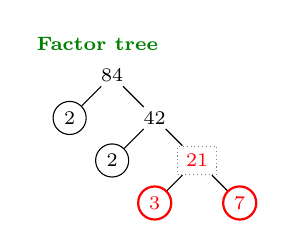
\begin{tikzpicture}[scale=0.9, every node/.style={font=\scriptsize}]
\node[dhead] at (-1.2,0.45) {\ealkey{Factor tree}};
\node[tnum]   (t84) at (0,0)       {$84$};
\node[tprime] (t2a) at (-0.6,-0.6) {$2$};
\node[tnum]   (t42) at (0.6,-0.6)  {$42$};
\node[tprime] (t2b) at (0,-1.2)    {$2$};
\node[tgap]   (t21) at (1.2,-1.2)  {};
\node[tpgap]  (t3)  at (0.6,-1.8)  {};
\node[tpgap]  (t7)  at (1.8,-1.8)  {};
\draw (t84) -- (t2a);  \draw (t84) -- (t42);
\draw (t42) -- (t2b);  \draw (t42) -- (t21);
\draw (t21) -- (t3);   \draw (t21) -- (t7);
\node[vans] at (t21) {$21$};
\node[tprime, ans] at (t3) {$3$};
\node[tprime, ans] at (t7) {$7$};
\end{tikzpicture}
\end{center}

\column{0.64\textwidth}
\vspace{-1.5em}
\footnotesize
\begin{enumerate}\tightlist
  \item \ealpara{\ealkeytr{Uprość} $\sqrt{20}$.}{\ealkey{Simplify} $\sqrt{20}$.}
        \ashow{$\sqrt{4\times5}=2\sqrt{5}$}
  \item \ealpara{Oblicz $2^{-1}$ i $9^{\frac12}$.}{Work out $2^{-1}$ and $9^{\frac12}$.}
        \ashow{$\dfrac12$ and $3$}
  \item \ealpara{Uzupełnij \ealkeytr{drzewko czynników}. Zapisz $84$ jako \ealkeytr{iloczyn} \ealkeytr{czynników pierwszych} w postaci z \ealkeytr{wykładnikami}.}{Complete the \ealkey{factor tree}. Write $84$ as a \ealkey{product} of \ealkey{prime factors} in \ealkey{index} form.}
        \ashow{$84=2^2\times3\times7$}
\end{enumerate}
\end{columns}
\end{frame}

\begin{frame}[t]{Starter 1: \ealkey{Prime Factors} \& \ealkey{HCF} (2 of 3)}
\begin{columns}[T,onlytextwidth]

\column{0.36\textwidth}
\begin{center}
\vspace{-0.6em}
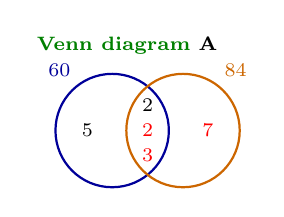
\begin{tikzpicture}[scale=0.9, every node/.style={font=\scriptsize}]
\node[dhead] at (-1.2,1.2) {\ealkey{Venn diagram} A};
\draw[vleft]  (0,0)   circle (0.8);
\draw[vright] (1.0,0) circle (0.8);
\node[vlabl] at (-0.45,0.85) {$60$};
\node[vlabr] at (1.45,0.85)  {$84$};
\node at (-0.35,0)   {$5$};
\node at (0.5,0.35)  {$2$};
\node[vans] at (0.5,0)     {$2$};
\node[vans] at (0.5,-0.35) {$3$};
\node[vans] at (1.35,0)    {$7$};
\end{tikzpicture}
\end{center}

\column{0.64\textwidth}
\vspace{-1.5em}
\footnotesize
\begin{enumerate}\tightlist
  \setcounter{enumi}{3}
  \item \ealpara{$60=2^2\times3\times5$. Uzupełnij \ealkeytr{diagram Venna} A dla $60$ i $84$, a następnie znajdź \ealkeytr{największy wspólny dzielnik} i \ealkeytr{najmniejszą wspólną wielokrotność} $60$ i $84$.}{$60=2^2\times3\times5$. Complete \ealkey{Venn diagram} A for $60$ and $84$, then find the \ealkey{HCF} and the \ealkey{LCM} of $60$ and $84$.}
        \ashow{\ealkey{HCF} $=12$; \; \ealkey{LCM} $=2^2\times3\times5\times7=420$}
  \item \ealpara{\ealkeytr{Uprość} $\dfrac{60}{84}$ dzieląc przez \ealkeytr{największy wspólny dzielnik}. Które liczby w \ealkeytr{diagramie Venna} A nie są w \ealkeytr{największym wspólnym dzielniku}?}{\ealkey{Simplify} $\dfrac{60}{84}$ by dividing by the \ealkey{HCF}. Which numbers in \ealkey{Venn diagram} A are not in the \ealkey{HCF}?}
        \ashow{$\dfrac{5}{7}$: the $5$ and the $7$, which are not shared}
\end{enumerate}
\end{columns}
\end{frame}

\begin{frame}[t]{Starter 1: \ealkey{Prime Factors} \& \ealkey{HCF} (3 of 3)}
\begin{columns}[T,onlytextwidth]

\column{0.36\textwidth}
\begin{center}
\vspace{-0.6em}
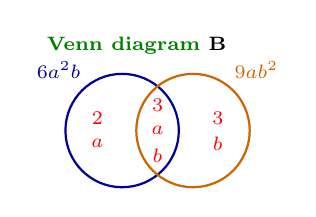
\begin{tikzpicture}[scale=0.9, every node/.style={font=\scriptsize}]
\node[dhead] at (-1.2,1.2) {\ealkey{Venn diagram} B};
\draw[vleft]  (0,0)   circle (0.8);
\draw[vright] (1.0,0) circle (0.8);
\node[vlabl] at (-0.45,0.85) {$6a^2b$};
\node[vlabr] at (1.45,0.85)  {$9ab^2$};
\node[vans] at (-0.35,0.18)  {$2$};
\node[vans] at (-0.35,-0.18) {$a$};
\node[vans] at (0.5,0.35)    {$3$};
\node[vans] at (0.5,0)       {$a$};
\node[vans] at (0.5,-0.35)   {$b$};
\node[vans] at (1.35,0.18)   {$3$};
\node[vans] at (1.35,-0.18)  {$b$};
\end{tikzpicture}
\end{center}

\column{0.64\textwidth}
\vspace{-1.5em}
\footnotesize
\begin{enumerate}\tightlist
  \setcounter{enumi}{5}
  \item \ealpara{\ealkeytr{Uprość} $\dfrac{x^5}{x^2}$ rozpisując $x$ i przez \ealkeytr{skracanie}.}{\ealkey{Simplify} $\dfrac{x^5}{x^2}$ by writing out the $x$s and \ealkey{cancelling}.}
        \ashow{$x^2$ \ealkey{cancels} from the top and the bottom, leaving $x^3=x^{5-2}$}
  \item \ealpara{(Wyzwanie) Uzupełnij \ealkeytr{diagram Venna} B dla $6a^2b$ i $9ab^2$. Użyj go, aby \ealkeytr{uprościć} $\dfrac{6a^2b}{9ab^2}$.}{(Challenge) Complete \ealkey{Venn diagram} B for $6a^2b$ and $9ab^2$. Use it to \ealkey{simplify} $\dfrac{6a^2b}{9ab^2}$.}
        \ashow{The \ealkey{HCF} is $3ab$, so $\dfrac{6a^2b}{9ab^2}=\dfrac{2a}{3b}$}
\end{enumerate}
\end{columns}
\end{frame}

\begin{frame}[t]{Starter 2: \ealkey{Index} Laws (1 of 3)}
\vspace{-1.5em}
\footnotesize
\begin{enumerate}\tightlist
  \item \ealpara{Zapisz $72$ jako \ealkeytr{iloczyn} \ealkeytr{czynników pierwszych} w postaci z \ealkeytr{wykładnikami}.}{Write $72$ as a \ealkey{product} of \ealkey{prime factors} in \ealkey{index} form.}
        \ashow{$72=2^3\times3^2$}
  \item \ealpara{\ealkeytr{Uprość} $\sqrt{8}+\sqrt{18}$.}{\ealkey{Simplify} $\sqrt{8}+\sqrt{18}$.}
        \ashow{$2\sqrt{2}+3\sqrt{2}=5\sqrt{2}$}
  \item \ealpara{\ealkeytr{Uprość} $x^4\times x^3$ i $y^8\div y^2$.}{\ealkey{Simplify} $x^4\times x^3$ and $y^8\div y^2$.}
        \ashow{$x^7$ and $y^6$}
\end{enumerate}
\end{frame}

\begin{frame}[t]{Starter 2: \ealkey{Index} Laws (2 of 3)}
\begin{columns}[T,onlytextwidth]

\column{0.36\textwidth}
\begin{center}
\vspace{-0.6em}
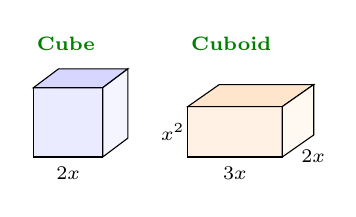
\begin{tikzpicture}[scale=0.8, every node/.style={font=\scriptsize}]
\node[dhead] at (-0.1,1.8) {\ealkey{Cube}};
\draw[fill=blue!8]  (0,0) rectangle (1.1,1.1);
\draw[fill=blue!16] (0,1.1) -- (0.4,1.4) -- (1.5,1.4) -- (1.1,1.1) -- cycle;
\draw[fill=blue!4]  (1.1,0) -- (1.5,0.3) -- (1.5,1.4) -- (1.1,1.1) -- cycle;
\node[below] at (0.55,0) {$2x$};

\begin{scope}[xshift=2.45cm]
\node[dhead] at (-0.1,1.8) {\ealkey{Cuboid}};
\draw[fill=orange!10] (0,0) rectangle (1.5,0.8);
\draw[fill=orange!20] (0,0.8) -- (0.5,1.15) -- (2.0,1.15) -- (1.5,0.8) -- cycle;
\draw[fill=orange!5]  (1.5,0) -- (2.0,0.35) -- (2.0,1.15) -- (1.5,0.8) -- cycle;
\node[below] at (0.75,0) {$3x$};
\node[left, inner sep=1pt] at (0,0.4) {$x^2$};
\node[below right, inner sep=1pt] at (1.75,0.17) {$2x$};
\end{scope}
\end{tikzpicture}
\end{center}

\column{0.64\textwidth}
\vspace{-1.5em}
\footnotesize
\begin{enumerate}\tightlist
  \setcounter{enumi}{3}
  \item \ealpara{Zapisz $2^{-3}$ i $x^{-2}$ jako \ealkeytr{ułamki}.}{Write $2^{-3}$ and $x^{-2}$ as \ealkey{fractions}.}
        \ashow{$\dfrac18$ and $\dfrac{1}{x^2}$}
  \item \ealpara{Znajdź \ealkeytr{objętość} \ealkeytr{sześcianu}. Czy to $2x^3$ czy $8x^3$?}{Find the \ealkey{volume} of the \ealkey{cube}. Is it $2x^3$ or $8x^3$?}
        \ashow{$(2x)^3=2^3x^3=8x^3$}
  \item \ealpara{Znajdź \ealkeytr{objętość} \ealkeytr{prostopadłościanu}.}{Find the \ealkey{volume} of the \ealkey{cuboid}.}
        \ashow{$3x\times2x\times x^2=6x^4$}
\end{enumerate}
\end{columns}
\end{frame}

\begin{frame}[t]{Starter 2: \ealkey{Index} Laws (3 of 3)}
\begin{columns}[T,onlytextwidth]

\column{0.36\textwidth}
\begin{center}
\vspace{-0.6em}
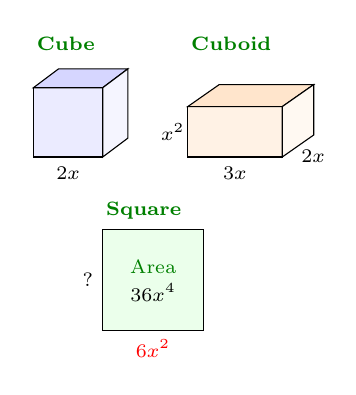
\begin{tikzpicture}[scale=0.8, every node/.style={font=\scriptsize}]
\node[dhead] at (-0.1,1.8) {\ealkey{Cube}};
\draw[fill=blue!8]  (0,0) rectangle (1.1,1.1);
\draw[fill=blue!16] (0,1.1) -- (0.4,1.4) -- (1.5,1.4) -- (1.1,1.1) -- cycle;
\draw[fill=blue!4]  (1.1,0) -- (1.5,0.3) -- (1.5,1.4) -- (1.1,1.1) -- cycle;
\node[below] at (0.55,0) {$2x$};

\begin{scope}[xshift=2.45cm]
\node[dhead] at (-0.1,1.8) {\ealkey{Cuboid}};
\draw[fill=orange!10] (0,0) rectangle (1.5,0.8);
\draw[fill=orange!20] (0,0.8) -- (0.5,1.15) -- (2.0,1.15) -- (1.5,0.8) -- cycle;
\draw[fill=orange!5]  (1.5,0) -- (2.0,0.35) -- (2.0,1.15) -- (1.5,0.8) -- cycle;
\node[below] at (0.75,0) {$3x$};
\node[left, inner sep=1pt] at (0,0.4) {$x^2$};
\node[below right, inner sep=1pt] at (1.75,0.17) {$2x$};
\end{scope}

\begin{scope}[xshift=1.1cm, yshift=-2.75cm]
\node[dhead] at (-0.1,1.9) {\ealkey{Square}};
\draw[fill=green!8] (0,0) rectangle (1.6,1.6);
\node at (0.8,1.0)  {\ealkey{Area}};
\node at (0.8,0.6)  {$36x^4$};
\node[left] at (0,0.8) {$?$};
\node[vans, below] at (0.8,0) {$6x^2$};
\end{scope}
\end{tikzpicture}
\end{center}

\column{0.64\textwidth}
\vspace{-1.5em}
\footnotesize
\begin{enumerate}\tightlist
  \setcounter{enumi}{6}
  \item \ealpara{\ealkeytr{Kwadrat} ma \ealkeytr{pole} $36x^4$, więc jego długość boku wynosi $\left(36x^4\right)^{\frac12}$. \ealkeytr{Uprość} to.}{The \ealkey{square} has \ealkey{area} $36x^4$, so its side length is $\left(36x^4\right)^{\frac12}$. \ealkey{Simplify} this.}
        \ashow{$36^{\frac12}\times x^{4\times\frac12}=6x^2$}
  \item \ealpara{(Rozszerzenie) Uzupełnij obliczenia.\\[2pt]
        \hspace*{1em}$8^{-\frac23}=\dfrac{1}{8^{\frac23}}=\dfrac{1}{\left(\sqrt[3]{8}\right)^2}
        =\dfrac{1}{\abox{$2$}^{\,2}}=\abox{$\dfrac14$}$}{(Extension) Complete the working.\\[2pt]
        \hspace*{1em}$8^{-\frac23}=\dfrac{1}{8^{\frac23}}=\dfrac{1}{\left(\sqrt[3]{8}\right)^2}
        =\dfrac{1}{\abox{$2$}^{\,2}}=\abox{$\dfrac14$}$}
  \item \ealpara{(Wyzwanie) Podziel \ealkeytr{objętość} \ealkeytr{sześcianu} przez \ealkeytr{objętość} \ealkeytr{prostopadłościanu}. Zapisz odpowiedź jako \ealkeytr{ułamek} w \ealkeytr{najprostszej postaci}.}{(Challenge) Divide the \ealkey{volume} of the \ealkey{cube} by the \ealkey{volume} of the \ealkey{cuboid}. Write the answer as a \ealkey{fraction} in its \ealkey{simplest form}.}
        \ashow{$\dfrac{8x^3}{6x^4}=\dfrac{4}{3x}$}
\end{enumerate}
\end{columns}
\end{frame}

\begin{frame}[t]{Starter 3: \ealkey{Surds} \& Single \ealkey{Brackets} (1 of 3)}
\begin{columns}[T,onlytextwidth]

\column{0.38\textwidth}
\begin{center}
\vspace{-0.6em}
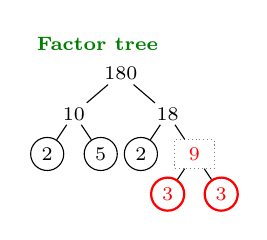
\begin{tikzpicture}[scale=0.85, every node/.style={font=\scriptsize}]
\node[dhead] at (-1.4,0.45) {\ealkey{Factor tree}};
\node[tnum]   (r)  at (0,0)        {$180$};
\node[tnum]   (a)  at (-0.7,-0.6)  {$10$};
\node[tnum]   (b)  at (0.7,-0.6)   {$18$};
\node[tprime] (a1) at (-1.1,-1.2)  {$2$};
\node[tprime] (a2) at (-0.3,-1.2)  {$5$};
\node[tprime] (b1) at (0.3,-1.2)   {$2$};
\node[tgap]   (b2) at (1.1,-1.2)   {};
\node[tpgap]  (c1) at (0.7,-1.8)   {};
\node[tpgap]  (c2) at (1.5,-1.8)   {};
\draw (r) -- (a);   \draw (r) -- (b);
\draw (a) -- (a1);  \draw (a) -- (a2);
\draw (b) -- (b1);  \draw (b) -- (b2);
\draw (b2) -- (c1); \draw (b2) -- (c2);
\node[vans] at (b2) {$9$};
\node[tprime, ans] at (c1) {$3$};
\node[tprime, ans] at (c2) {$3$};
\end{tikzpicture}
\end{center}

\column{0.62\textwidth}
\vspace{-1.5em}
\footnotesize
\begin{enumerate}\tightlist
  \item \ealpara{Znajdź \ealkeytr{największy wspólny dzielnik} $18$ i $24$.}{Find the \ealkey{HCF} of $18$ and $24$.}
        \ashow{$6$}
  \item \ealpara{Oblicz $16^{\frac12}$ i $16^{-\frac12}$.}{Work out $16^{\frac12}$ and $16^{-\frac12}$.}
        \ashow{$4$ and $\dfrac14$}
  \item \ealpara{Uzupełnij \ealkeytr{drzewko czynników}. Zapisz $180$ jako \ealkeytr{iloczyn} \ealkeytr{czynników pierwszych} w postaci z \ealkeytr{wykładnikami}.}{Complete the \ealkey{factor tree}. Write $180$ as a \ealkey{product} of \ealkey{prime factors} in \ealkey{index} form.}
        \ashow{$180=2^2\times3^2\times5$}
\end{enumerate}
\end{columns}
\end{frame}

\begin{frame}[t]{Starter 3: \ealkey{Surds} \& Single \ealkey{Brackets} (2 of 3)}
\begin{columns}[T,onlytextwidth]

\column{0.38\textwidth}
\begin{center}
\vspace{-0.6em}
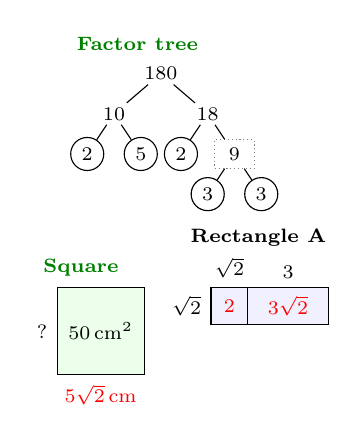
\begin{tikzpicture}[scale=0.85, every node/.style={font=\scriptsize}]
\node[dhead] at (-1.4,0.45) {\ealkey{Factor tree}};
\node[tnum]   (r)  at (0,0)        {$180$};
\node[tnum]   (a)  at (-0.7,-0.6)  {$10$};
\node[tnum]   (b)  at (0.7,-0.6)   {$18$};
\node[tprime] (a1) at (-1.1,-1.2)  {$2$};
\node[tprime] (a2) at (-0.3,-1.2)  {$5$};
\node[tprime] (b1) at (0.3,-1.2)   {$2$};
\node[tgap]   (b2) at (1.1,-1.2)   {};
\node[tpgap]  (c1) at (0.7,-1.8)   {};
\node[tpgap]  (c2) at (1.5,-1.8)   {};
\draw (r) -- (a);   \draw (r) -- (b);
\draw (a) -- (a1);  \draw (a) -- (a2);
\draw (b) -- (b1);  \draw (b) -- (b2);
\draw (b2) -- (c1); \draw (b2) -- (c2);
\node at (b2) {$9$};
\node[tprime] at (c1) {$3$};
\node[tprime] at (c2) {$3$};

\begin{scope}[xshift=-1.55cm, yshift=-4.5cm]
\node[dhead] at (-0.35,1.6) {\ealkey{Square}};
\draw[fill=green!8] (0,0) rectangle (1.3,1.3);
\node at (0.65,0.65) {$50$\,cm$^2$};
\node[left] at (0,0.65) {$?$};
\node[vans, below] at (0.65,0) {$5\sqrt{2}$\,cm};
\end{scope}

\begin{scope}[xshift=0.75cm, yshift=-3.75cm]
\node[dhead] at (-0.45,1.3) {Rectangle A};
\draw[fill=blue!6] (0,0) rectangle (0.55,0.55);
\draw[fill=blue!6] (0.55,0) rectangle (1.75,0.55);
\node[above] at (0.275,0.55) {$\sqrt{2}$};
\node[above] at (1.15,0.55)  {$3$};
\node[left]  at (0,0.275)    {$\sqrt{2}$};
\node[vans] at (0.275,0.275) {$2$};
\node[vans] at (1.15,0.275)  {$3\sqrt{2}$};
\end{scope}
\end{tikzpicture}
\end{center}

\column{0.62\textwidth}
\vspace{-1.5em}
\footnotesize
\begin{enumerate}\tightlist
  \setcounter{enumi}{3}
  \item \ealpara{Użyj \ealkeytr{czynników pierwszych}, aby \ealkeytr{uprościć} $\sqrt{180}$.}{Use the \ealkey{prime factors} to \ealkey{simplify} $\sqrt{180}$.}
        \ashow{$\sqrt{2^2\times3^2\times5}=2\times3\times\sqrt{5}=6\sqrt{5}$}
  \item \ealpara{\ealkeytr{Kwadrat} ma \ealkeytr{pole} $50$\,cm$^2$. Znajdź długość jego boku jako uproszczony \ealkeytr{pierwiastek niewymierny} oraz jego \ealkeytr{obwód}.}{The \ealkey{square} has \ealkey{area} $50$\,cm$^2$. Find its side length as a simplified \ealkey{surd}, and its \ealkey{perimeter}.}
        \ashow{$\sqrt{50}=5\sqrt{2}$\,cm; \; $4\times5\sqrt{2}=20\sqrt{2}$\,cm}
  \item \ealpara{Uzupełnij prostokąt A, aby \ealkeytr{wymnożyć nawiasy} $\sqrt{2}(\sqrt{2}+3)$.}{Complete rectangle A to \ealkey{expand} $\sqrt{2}(\sqrt{2}+3)$.}
        \ashow{$2+3\sqrt{2}$}
\end{enumerate}
\end{columns}
\end{frame}

\begin{frame}[t]{Starter 3: \ealkey{Surds} \& Single \ealkey{Brackets} (3 of 3)}
\begin{columns}[T,onlytextwidth]

\column{0.38\textwidth}
\begin{center}
\vspace{-0.6em}
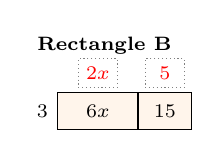
\begin{tikzpicture}[scale=0.85, every node/.style={font=\scriptsize}]
\begin{scope}[xshift=0.75cm, yshift=-0.5cm]
\node[dhead] at (-0.45,1.25) {Rectangle B};
\draw[fill=orange!8] (0,0) rectangle (1.2,0.55);
\draw[fill=orange!8] (1.2,0) rectangle (2.0,0.55);
\node[tgap] (bl) at (0.6,0.84) {};
\node[tgap] (br) at (1.6,0.84) {};
\node[left] at (0,0.275) {$3$};
\node at (0.6,0.275) {$6x$};
\node at (1.6,0.275) {$15$};
\node[vans] at (bl) {$2x$};
\node[vans] at (br) {$5$};
\end{scope}
\end{tikzpicture}
\end{center}

\column{0.62\textwidth}
\vspace{-1.5em}
\footnotesize
\begin{enumerate}\tightlist
  \setcounter{enumi}{6}
  \item \ealpara{Uzupełnij prostokąt B, aby \ealkeytr{rozłożyć na czynniki} $6x+15$. Następnie \ealkeytr{uprość} $\dfrac{6x+15}{3}$.}{Complete rectangle B to \ealkey{factorise} $6x+15$. Then \ealkey{simplify} $\dfrac{6x+15}{3}$.}
        \ashow{$3(2x+5)$; \; $2x+5$, not $2x+15$}
  \item \ealpara{(Wyzwanie) Sam mówi, że $\dfrac{6+\sqrt{18}}{3}=2+\sqrt{18}$. Wyjaśnij błąd Sama, a następnie \ealkeytr{uprość} to poprawnie.}{(Challenge) Sam says $\dfrac{6+\sqrt{18}}{3}=2+\sqrt{18}$. Explain Sam's mistake, then \ealkey{simplify} it correctly.}
        \ashow{Divide both terms by $3$: \; $2+\dfrac{3\sqrt{2}}{3}=2+\sqrt{2}$}
\end{enumerate}
\end{columns}
\end{frame}

\begin{frame}[t]{Starter 4: Double \ealkey{Brackets} (1 of 3)}
\begin{columns}[T,onlytextwidth]

\column{0.36\textwidth}
\begin{center}
\vspace{-0.6em}
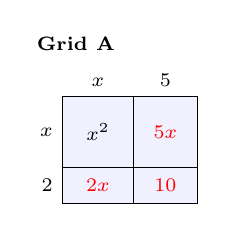
\begin{tikzpicture}[scale=0.9, every node/.style={font=\scriptsize}]
\node[dhead] at (-0.5,0.75) {Grid A};
\draw[fill=blue!6] (0,0)      rectangle (1.0,-1.0);
\draw[fill=blue!6] (1.0,0)    rectangle (1.9,-1.0);
\draw[fill=blue!6] (0,-1.0)   rectangle (1.0,-1.5);
\draw[fill=blue!6] (1.0,-1.0) rectangle (1.9,-1.5);
\node[above] at (0.5,0)     {$x$};
\node[above] at (1.45,0)    {$5$};
\node[left]  at (0,-0.5)    {$x$};
\node[left]  at (0,-1.25)   {$2$};
\node at (0.5,-0.5) {$x^2$};
\node[vans] at (1.45,-0.5)  {$5x$};
\node[vans] at (0.5,-1.25)  {$2x$};
\node[vans] at (1.45,-1.25) {$10$};
\end{tikzpicture}
\end{center}

\column{0.64\textwidth}
\vspace{-1.5em}
\footnotesize
\begin{enumerate}\tightlist
  \item \ealpara{Czy $3^{-2}$ równa się $-9$, $-6$ czy $\frac19$?}{Is $3^{-2}$ equal to $-9$, $-6$ or $\frac19$?}
        \ashow{$\dfrac{1}{3^2}=\dfrac19$}
  \item \ealpara{\ealkeytr{Uprość} $\sqrt{50}-\sqrt{8}$. Czy to $\sqrt{42}$?}{\ealkey{Simplify} $\sqrt{50}-\sqrt{8}$. Is it $\sqrt{42}$?}
        \ashow{No: $5\sqrt{2}-2\sqrt{2}=3\sqrt{2}$}
  \item \ealpara{Uzupełnij siatkę A, aby \ealkeytr{wymnożyć nawiasy} $(x+2)(x+5)$.}{Complete grid A to \ealkey{expand} $(x+2)(x+5)$.}
        \ashow{$x^2+7x+10$}
\end{enumerate}
\end{columns}
\end{frame}

\begin{frame}[t]{Starter 4: Double \ealkey{Brackets} (2 of 3)}
\begin{columns}[T,onlytextwidth]

\column{0.36\textwidth}
\begin{center}
\vspace{-0.6em}
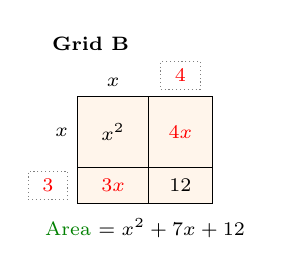
\begin{tikzpicture}[scale=0.9, every node/.style={font=\scriptsize}]
\node[dhead] at (-0.5,0.75) {Grid B};
\draw[fill=orange!8] (0,0)      rectangle (1.0,-1.0);
\draw[fill=orange!8] (1.0,0)    rectangle (1.9,-1.0);
\draw[fill=orange!8] (0,-1.0)   rectangle (1.0,-1.5);
\draw[fill=orange!8] (1.0,-1.0) rectangle (1.9,-1.5);
\node[above] at (0.5,0) {$x$};
\node[tgap] (gt) at (1.45,0.3) {};
\node[left]  at (0,-0.5) {$x$};
\node[tgap] (gl) at (-0.42,-1.25) {};
\node at (0.5,-0.5)   {$x^2$};
\node at (1.45,-1.25) {$12$};
\node[font=\scriptsize] at (0.95,-1.85) {\ealkey{Area} $=x^2+7x+12$};
\node[vans] at (gt) {$4$};
\node[vans] at (gl) {$3$};
\node[vans] at (1.45,-0.5) {$4x$};
\node[vans] at (0.5,-1.25) {$3x$};
\end{tikzpicture}
\end{center}

\column{0.64\textwidth}
\vspace{-1.5em}
\footnotesize
\begin{enumerate}\tightlist
  \setcounter{enumi}{3}
  \item \ealpara{Zapisz $12$ jako \ealkeytr{iloczyn} \ealkeytr{czynników pierwszych}, a następnie wypisz jego \ealkeytr{pary czynników}. Która para sumuje się do $7$?}{Write $12$ as a \ealkey{product} of \ealkey{prime factors}, then list its \ealkey{factor pairs}. Which pair adds to $7$?}
        \ashow{$2^2\times3$; \; $1\times12$, $2\times6$, $3\times4$; \; $3+4=7$}
  \item \ealpara{Uzupełnij siatkę B, aby \ealkeytr{rozłożyć na czynniki} $x^2+7x+12$.}{Complete grid B to \ealkey{factorise} $x^2+7x+12$.}
        \ashow{$(x+3)(x+4)$, in either order}
  \item \ealpara{Prostokąt ma \ealkeytr{pole} $x^2+7x+12$ i szerokość $x+3$. Znajdź jego długość. Użyj tego, aby \ealkeytr{uprościć} $\dfrac{x^2+7x+12}{x+3}$.}{A rectangle has \ealkey{area} $x^2+7x+12$ and width $x+3$. Find its length. Use this to \ealkey{simplify} $\dfrac{x^2+7x+12}{x+3}$.}
        \ashow{$\dfrac{(x+3)(x+4)}{x+3}=x+4$}
\end{enumerate}
\end{columns}
\end{frame}

\begin{frame}[t]{Starter 4: Double \ealkey{Brackets} (3 of 3)}
\vspace{-1.5em}
\footnotesize
\begin{enumerate}\tightlist
  \setcounter{enumi}{6}
  \item \ealpara{\ealkeytr{Rozłóż na czynniki} $x^2-9$. Użyj \ealkeytr{różnicy dwóch kwadratów}, aby \ealkeytr{wymnożyć nawiasy} $(3+\sqrt{2})(3-\sqrt{2})$.}{\ealkey{Factorise} $x^2-9$. Use the \ealkey{difference of two squares} to \ealkey{expand} $(3+\sqrt{2})(3-\sqrt{2})$.}
        \ashow{$(x+3)(x-3)$; \; $9-2=7$}
  \item \ealpara{(Wyzwanie) $391=20^2-3^2$. Użyj tego, aby zapisać $391$ jako \ealkeytr{iloczyn} \ealkeytr{czynników pierwszych}.}{(Challenge) $391=20^2-3^2$. Use this to write $391$ as a \ealkey{product} of \ealkey{prime factors}.}
        \ashow{$(20+3)(20-3)=23\times17$, both \ealkey{prime}}
\end{enumerate}
\end{frame}

\begin{frame}[t]{Starter 5: \ealkey{LCM} \& \ealkey{Fractions} (1 of 3)}
\begin{columns}[T,onlytextwidth]

\column{0.36\textwidth}
\begin{center}
\vspace{-0.6em}
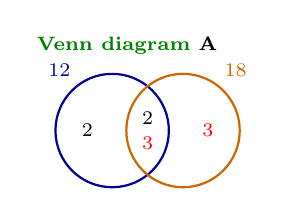
\begin{tikzpicture}[scale=0.9, every node/.style={font=\scriptsize}]
\node[dhead] at (-1.2,1.2) {\ealkey{Venn diagram} A};
\draw[vleft]  (0,0)   circle (0.8);
\draw[vright] (1.0,0) circle (0.8);
\node[vlabl] at (-0.45,0.85) {$12$};
\node[vlabr] at (1.45,0.85)  {$18$};
\node at (-0.35,0)  {$2$};
\node at (0.5,0.18) {$2$};
\node[vans] at (0.5,-0.18) {$3$};
\node[vans] at (1.35,0)    {$3$};
\end{tikzpicture}
\end{center}

\column{0.64\textwidth}
\vspace{-1.5em}
\footnotesize
\begin{enumerate}\tightlist
  \item \ealpara{\ealkeytr{Uprość} $a^3\times a^{-1}$.}{\ealkey{Simplify} $a^3\times a^{-1}$.}
        \ashow{$a^{3+(-1)}=a^2$}
  \item \ealpara{Oblicz $\sqrt{8}\times\sqrt{2}$.}{Work out $\sqrt{8}\times\sqrt{2}$.}
        \ashow{$\sqrt{16}=4$}
  \item \ealpara{$12=2^2\times3$ i $18=2\times3^2$. Uzupełnij \ealkeytr{diagram Venna} A, a następnie znajdź \ealkeytr{największy wspólny dzielnik} i \ealkeytr{najmniejszą wspólną wielokrotność} $12$ i $18$.}{$12=2^2\times3$ and $18=2\times3^2$. Complete \ealkey{Venn diagram} A, then find the \ealkey{HCF} and the \ealkey{LCM} of $12$ and $18$.}
        \ashow{\ealkey{HCF} $=6$; \; \ealkey{LCM} $=2^2\times3^2=36$}
\end{enumerate}
\end{columns}
\end{frame}

\begin{frame}[t]{Starter 5: \ealkey{LCM} \& \ealkey{Fractions} (2 of 3)}
\vspace{-1.5em}
\footnotesize
\begin{enumerate}\tightlist
  \setcounter{enumi}{3}
  \item \ealpara{Uzupełnij: $\dfrac{5}{12}+\dfrac{7}{18}=\dfrac{\abox{$15$}}{36}+\dfrac{\abox{$14$}}{36}=\dfrac{\abox{$29$}}{36}$}{Complete: $\dfrac{5}{12}+\dfrac{7}{18}=\dfrac{\abox{$15$}}{36}+\dfrac{\abox{$14$}}{36}=\dfrac{\abox{$29$}}{36}$}
  \item \ealpara{Zapisz $\dfrac{x}{12}-\dfrac{x}{18}$ jako pojedynczy \ealkeytr{ułamek}.}{Write $\dfrac{x}{12}-\dfrac{x}{18}$ as a single \ealkey{fraction}.}
        \ashow{$\dfrac{3x}{36}-\dfrac{2x}{36}=\dfrac{x}{36}$}
  \item \ealpara{Oblicz $\dfrac34\times\dfrac89$. Następnie \ealkeytr{uprość} $\dfrac{3x}{4}\div\dfrac{9x}{10}$.}{Work out $\dfrac34\times\dfrac89$. Then \ealkey{simplify} $\dfrac{3x}{4}\div\dfrac{9x}{10}$.}
        \ashow{$\dfrac{24}{36}=\dfrac23$; \;
               $\dfrac{3x}{4}\times\dfrac{10}{9x}=\dfrac{30x}{36x}=\dfrac56$}
\end{enumerate}
\end{frame}

\begin{frame}[t]{Starter 5: \ealkey{LCM} \& \ealkey{Fractions} (3 of 3)}
\begin{columns}[T,onlytextwidth]

\column{0.36\textwidth}
\begin{center}
\vspace{-0.6em}
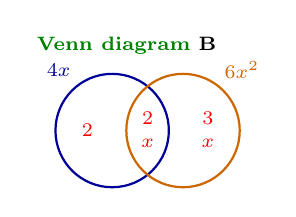
\begin{tikzpicture}[scale=0.9, every node/.style={font=\scriptsize}]
\node[dhead] at (-1.2,1.2) {\ealkey{Venn diagram} B};
\draw[vleft]  (0,0)   circle (0.8);
\draw[vright] (1.0,0) circle (0.8);
\node[vlabl] at (-0.45,0.85) {$4x$};
\node[vlabr] at (1.45,0.85)  {$6x^2$};
\node[vans] at (-0.35,0)     {$2$};
\node[vans] at (0.5,0.18)    {$2$};
\node[vans] at (0.5,-0.18)   {$x$};
\node[vans] at (1.35,0.18)   {$3$};
\node[vans] at (1.35,-0.18)  {$x$};
\end{tikzpicture}
\end{center}

\column{0.64\textwidth}
\vspace{-1.5em}
\footnotesize
\begin{enumerate}\tightlist
  \setcounter{enumi}{6}
  \item \ealpara{$4x=2\times2\times x$ i $6x^2=2\times3\times x\times x$. Uzupełnij \ealkeytr{diagram Venna} B, a następnie znajdź \ealkeytr{najmniejszą wspólną wielokrotność} $4x$ i $6x^2$.}{$4x=2\times2\times x$ and $6x^2=2\times3\times x\times x$. Complete \ealkey{Venn diagram} B, then find the \ealkey{LCM} of $4x$ and $6x^2$.}
        \ashow{$2\times2\times3\times x\times x=12x^2$}
  \item \ealpara{(Wyzwanie) Zapisz $\dfrac{5}{4x}+\dfrac{1}{6x^2}$ jako pojedynczy \ealkeytr{ułamek}.}{(Challenge) Write $\dfrac{5}{4x}+\dfrac{1}{6x^2}$ as a single \ealkey{fraction}.}
        \ashow{$\dfrac{15x}{12x^2}+\dfrac{2}{12x^2}=\dfrac{15x+2}{12x^2}$}
\end{enumerate}
\end{columns}
\end{frame}

\end{document}